\documentclass[a4paper]{scrartcl}
\usepackage[utf8]{inputenc}
% \usepackage{showframe} % disable this to hide #border.
\usepackage{wrapfig}
% Example:
% \begin{wrapfigure}{R}{0.4\textwidth}
% \centering
% 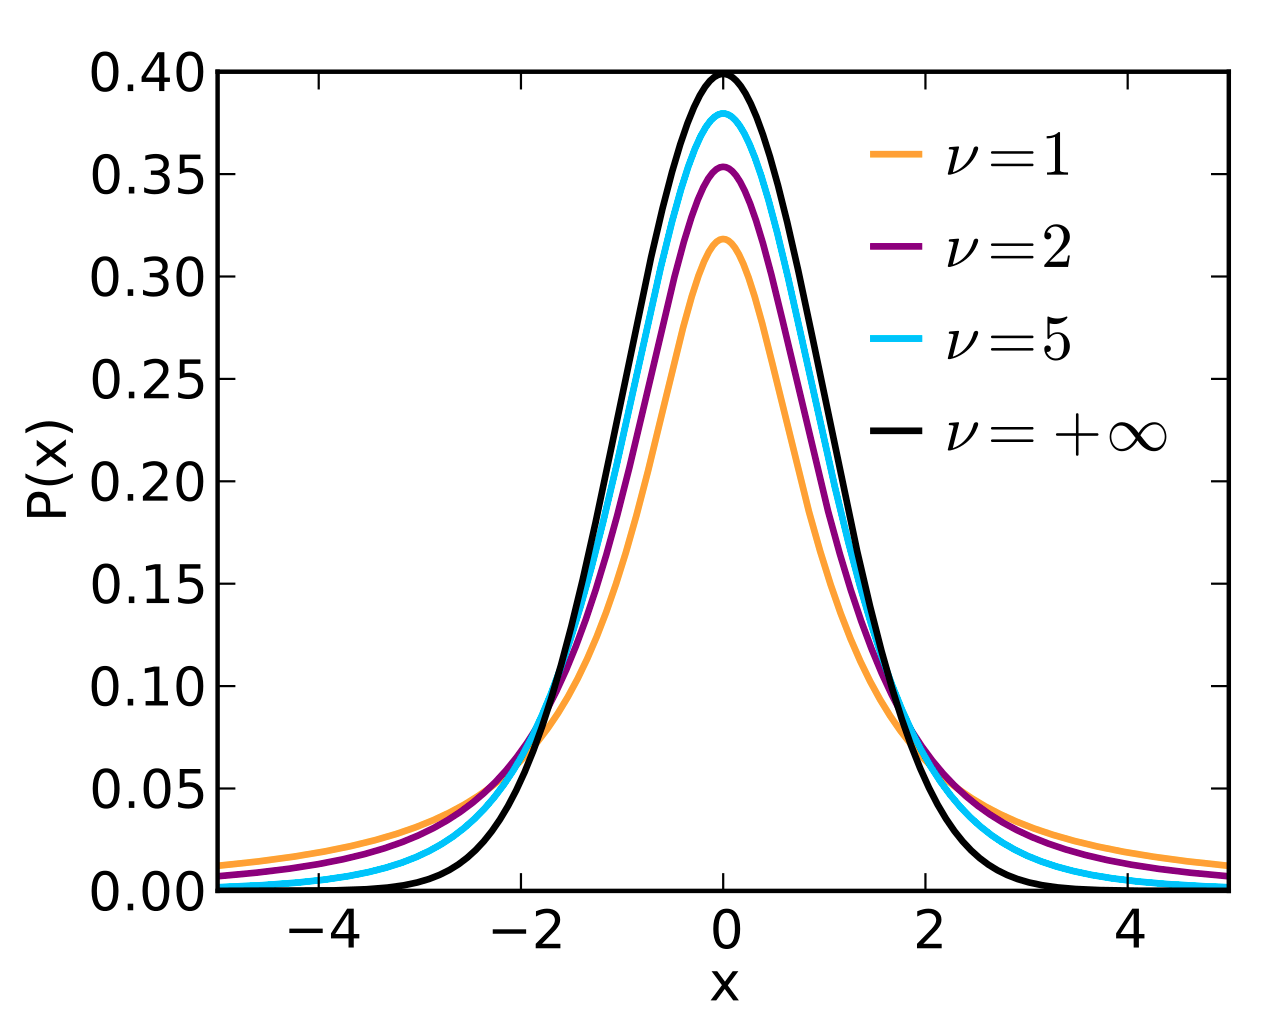
\includegraphics[width=0.35\textwidth]{assets/lectures_part_3-91d0349d.png}
% The PDF of the Student distribution.
% \end{wrapfigure}


\usepackage[english, russian, ukrainian]{babel}
\usepackage{misccorr,
            color,
            ragged2e,
            amsfonts,
            amsthm,
            graphicx,
            systeme,
            amsmath,
            mdframed,
            lipsum,
            mathtools,
            setspace
            }

\renewcommand\qedsymbol{$\blacksquare$}
\renewcommand*{\proofname}{\text{Доведення}}

\theoremstyle{definition}
\newtheorem*{defo}{Означення}
\newtheorem*{lemme}{Лема}
\newtheorem*{example}{Приклад}
\theoremstyle{remark}
\newtheorem*{remark}{Зауваження}
\theoremstyle{definition}
\newtheorem*{consequence}{Наслідок}
\theoremstyle{definition}
\newtheorem{statement}{Твердження}[section]
\newmdtheoremenv{boxteo}{Теорема}[section]

\setlength{\parindent}{0em}
\setlength{\parskip}{0.5em}
\DeclareMathOperator*\lowlim{\underline{lim}}
\DeclareMathOperator*\uplim{\overline{lim}}

\newcommand\independent{\protect\mathpalette{\protect\independenT}{\perp}}
\def\independenT#1#2{\mathrel{\rlap{$#1#2$}\mkern2mu{#1#2}}}

\usepackage{tikz}
\newcommand*\circled[1]{\tikz[baseline=(char.base)]{
  \node[shape=circle,draw,inner sep=1pt] (char) {#1};}}

% Default fixed font does not support bold face
\DeclareFixedFont{\ttb}{T1}{txtt}{bx}{n}{12} % for bold
\DeclareFixedFont{\ttm}{T1}{txtt}{m}{n}{12}  % for normal

% Custom colors
\definecolor{deepblue}{rgb}{0,0,0.5}
\definecolor{deepred}{rgb}{0.6,0,0}
\definecolor{deepgreen}{rgb}{0,0.5,0}

\usepackage{listings}

% Python style for highlighting
\newcommand\pythonstyle{\lstset{
language=Python,
basicstyle=\ttm,
morekeywords={self},              % Add keywords here
keywordstyle=\ttb\color{deepblue},
emph={MyClass,__init__},          % Custom highlighting
emphstyle=\ttb\color{deepred},    % Custom highlighting style
stringstyle=\color{deepgreen},
frame=tb,                         % Any extra options here
showstringspaces=false
}}


% Python environment
\lstnewenvironment{python}[1][]
{
\pythonstyle
\lstset{#1}
}
{}

% Python for external files
\newcommand\pythonexternal[2][]{{
\pythonstyle
\lstinputlisting[#1]{#2}}}

% Python for inline
\newcommand\pythoninline[1]{{\pythonstyle\lstinline!#1!}}

%                 USAGE:
% \begin{python}
% class MyClass(Yourclass):
%     def __init__(self, my, yours):
%         bla = '5 1 2 3 4'
%         print bla
% \end{python}
%
%
% \pythonexternal{demo.py}
%
%
% Definition \pythoninline{class MyClass} means \dots

\def\be{\begin{equation}}      % equation
\def\ee{\end{equation}}        % ...
\def\i{\infty}                 % infinity
\def\d{\partial}               % dx dy - partial     = \d
\def\bdash{\ \Big|\  }         % big vertical line   = |
\def\index{\mathbb{I}}         % indicator
\def\res#1{\underset{#1}{\mathrm{res}}}

% ^^^^^^^^^^^^^^^^^^^^^^^^^^^^^^^
\newcommand\reallywidehat[1]{\arraycolsep=0pt\relax%
\begin{array}{c}
\stretchto{
  \scaleto{
    \scalerel*[\widthof{\ensuremath{#1}}]{\kern-.5pt\bigwedge\kern-.5pt}
    {\rule[-\textheight/2]{1ex}{\textheight}} %WIDTH-LIMITED BIG WEDGE
  }{\textheight} %
}{0.5ex}\\           % THIS SQUEEZES THE WEDGE TO 0.5ex HEIGHT
#1\\                 % THIS STACKS THE WEDGE ATOP THE ARGUMENT
\rule{-1ex}{0ex}
\end{array}
}

\begin{document}

\tableofcontents
\newpage

\begin{center}
	\Huge \textbf{Ряд Фур'є}
\end{center}
\par
\section{Ряди Фур'є.}
\subsection{Поява. Передмова.}
Нехай $g(z)$ -- аналітична в  кільці $K = \left\lbrace  z \bdash 1 - \varepsilon_1 < |z| < 1 + \varepsilon_2 \right\rbrace$; $ \left\lbrace  z \bdash  |z| = 1 \right\rbrace \subset K.$\par
Розкладаємо $g(z)$ в ряд Лорана за степенями $z $ в цьому кільці:
$$
g(z) =  \sum\limits_{n =  - \i}^{ \infty}{ C_n \cdot z^n} \text{ , де } C_n = \frac{1}{2\pi i}  \int\limits_{|z| = 1 }^{ }{ \frac{ g(z)}{z^{n+1} }  \mathrm{d} z}
$$
$$
z : |z| =1 \ \Longrightarrow \  z = e^{ix} \ \Longrightarrow \  x \in  [0, 2 \pi]
 \ \Longrightarrow \
g(z) = g(e^{ix}) = f(x)
$$
$$
C_n = \frac{1}{2\pi i}  \int\limits_{|z| = 1 }^{ }{ \frac{ g(z)}{z^{n+1} }  \mathrm{d} z} = \left|  \begin{gathered}
  z = e^{ix}\\
  \mathrm{d} z = ie^{ix} \mathrm{d} x \\
  x \in [0, 2\pi]
\end{gathered} \right| = \frac{1}{2\pi}  \int\limits_{0}^{ 2 \pi}{ f(x) e^{-inx} \mathrm{d} x}
$$
Отримали \textit{комплексну форму ряду Фур'є}:
$$
f(x) =  \sum\limits_{n =-\i }^{ \infty}{C_n \cdot e^{inx}}, \  C_n =  \frac{1}{2\pi}  \int\limits_{0}^{ 2 \pi}{ f(x) e^{-inx} \mathrm{d} x}
$$
\subsection{Комплексна форма ряду Фур'є.}
$f \in D[0, 2\pi]$ -- періодична, інтегрова на $[0, 2 \pi]$. За функцією $f(x)$ будуємо ряд Фур'є:
$$
S(x) =  \sum\limits_{n =-\i }^{ \infty}{C_n \cdot e^{inx}}, \  C_n =  \frac{1}{2\pi}  \int\limits_{0}^{ 2 \pi}{ f(x) e^{-inx} \mathrm{d} x}
$$
Питання:
\begin{enumerate}
  \item  Збіжність ряду.
\item  Якщо збігається, то зв'язок між $S(x)$ та $f(x)$.
\end{enumerate}
\subsection{Випадок дійснозначної функції.}
Розглянемо ряд Фур'є:
$$
 \sum\limits_{n = -\infty}^{ -1}{C_n \cdot e^{inx}} + C_0 +  \sum\limits_{n = 1}^{ \infty}{C_n e^{inx}} = \left| \begin{gathered}
  \text{в І сумі:}\\
  n= -k
 \end{gathered} \right| =  \sum\limits_{k = 1}^{ \infty}{C_{-k} \cdot e^{-ikx}} + C_0 +  \sum\limits_{n = 1}^{ \infty}{C_n e^{inx}} \ \circled{=}
$$
Окремо розглянемо $C_{-k} e^{-ikx}$: $C_{-k} e^{-ikx} = \overline{C_{k} e^{ikx}}$:
$$
\circled{=} \ C_0 +  \sum\limits_{n = 1}^{ \infty}{\underbrace{\left( C_n e^{inx} + \overline{C_n e^{inx}} \right)}_{ = 2 \Re(C_n e^{inx})\in \mathbb{R}}} \ \fbox{$=$}
$$
$$
C_n = \frac{1}{2\pi}  \int\limits_{0}^{ 2 \pi}{ f(x) e^{-inx} \mathrm{d} x} = \frac{1}{2 \pi}   \int\limits_{0}^{ 2 \pi}{ f(x) \cdot \left( \cos{(nx)} - i \sin{(nx)} \right) \mathrm{d} x} =
$$
$$
 = \frac{1}{2\pi} \int\limits_{0}^{ 2 \pi}{ f(x) \cdot  \cos{(nx)} \mathrm{d} x} - i\frac{1}{2\pi}  \int\limits_{0}^{ 2 \pi}{ f(x) \cdot  \sin{(nx)} \mathrm{d} x}
$$
$$
 \Re C_n e^{inx} \!=\! \Re \left[ \frac{1}{2\pi}\!\int\limits_{0}^{ 2 \pi}{ f(x)  \cos{(nx)} \mathrm{d} x} - i \frac{1}{2\pi}\! \int\limits_{0}^{ 2 \pi}{ f(x)  \sin{(nx)} \mathrm{d} x}  \right] \cdot \left( \cos{(nx)} + i \sin{(nx)} \right)\! =
$$
$$
= \frac{1}{2\pi} \cos{(nx)} \int\limits_{0}^{ 2 \pi}{ f(x) \cdot  \cos{(nx)} \mathrm{d} x} + \frac{1}{2\pi}\sin{(nx)}  \int\limits_{0}^{ 2 \pi}{ f(x) \cdot  \sin{(nx)} \mathrm{d} x}
$$
$$
\fbox{$=$} \  C_0 +  \frac{1}{\pi} \sum\limits_{n = 1}^{ \infty}{
 \cos{(nx)} \int\limits_{0}^{ 2 \pi}{ f(x) \cdot  \cos{(nx)} \mathrm{d} x} + \sin{(nx)}  \int\limits_{0}^{ 2 \pi}{ f(x) \cdot  \sin{(nx)} \mathrm{d} x}
}
$$
$$
 C_0 = \frac{1}{2\pi}  \int\limits_{0}^{2\pi}{ f(x)dx} \qquad \quad \text{ Отримали} \textit{ дійсну форму ряда Фур'є.}
$$
$$
f(x) \mapsto \frac{a_0}{2} +  \sum\limits_{n = 1 }^{ \infty}{a_n \cos{( nx)} + b_n \sin{(nx)}},
$$
де $
a_n = \frac{1}{\pi}  \int\limits_{0}^{ 2\pi}{f(x) \cos{(nx)} \mathrm{d} x} , n \in \mathbb{N}\cup \left\lbrace 0 \right\rbrace ; \  b_n = \frac{1}{\pi}  \int\limits_{0}^{ 2\pi}{f(x) \sin{(nx)} \mathrm{d} x}, n \in \mathbb{N}\cup \left\lbrace 0 \right\rbrace.
$
\newpage

\subsection{Не $2\pi$-періодичні функції.}
$f$  -- $2l$ періодична, або задана на $[0, 2l]$, інтегрована. Розглянемо відображення:
$$
[0, 2\pi] \leftarrow [0, 2l] \qquad x \in [0, 2\pi] \qquad x = \frac{t}{l}\pi \qquad t\in [0, 2\pi]
$$
Тоді $f(x) = f( \frac{t}{l}\pi ) = g(t)$. $g(t)$ - задана на $[0, 2\l]$.
$$
a_n = \frac{1}{\pi}  \int\limits_{0}^{2\pi}{ f(x) \cos{(nx)} \mathrm{d} x } =   \frac{1
}{l }  \int\limits_{0}^{2l}{ g(t) \cos{ \left( \frac{\pi n t}{l}  \right)} \mathrm{d} t}
$$
$$
b_n = \frac{1}{\pi}  \int\limits_{0}^{2\pi}{ f(x) \sin{(nx)} \mathrm{d} x } =   \frac{1
}{l }  \int\limits_{0}^{2l}{ g(t) \sin{ \left( \frac{\pi n t}{l}  \right)} \mathrm{d} t}
$$
$$
g(t) = f(x) \mapsto \frac{a_0}{2} +  \sum\limits_{n = 1}^{ \infty}{a_n \cos{ \left(  \frac{\pi n t}{l} + b_n\sin{ \left( \frac{\pi n t}{l}  \right)}   \right)}}
$$
$$
a_n =\frac{1
}{l }  \int\limits_{0}^{2l}{ g(t) \cos{ \left( \frac{\pi n t}{l}  \right)} \mathrm{d} t}
 \qquad b_n = \frac{1
}{l }  \int\limits_{0}^{2l}{ g(t) \sin{ \left( \frac{\pi n t}{l}  \right)} \mathrm{d} t}
$$
Частіше всього, зручно обчислювати коефіцієнти ряду інакше:
$$
a_n =\frac{1
}{l }  \int\limits_{-l}^{l}{ g(t) \cos{ \left( \frac{\pi n t}{l}  \right)} \mathrm{d} t}
 \qquad b_n = \frac{1
}{l }  \int\limits_{-l}^{l}{ g(t) \sin{ \left( \frac{\pi n t}{l}  \right)} \mathrm{d} t}
$$
\newpage
\subsection{Аналіз збіжності ряду.}
\begin{lemme}[Рімана]
$f$ -- інтегрована на $[a,b]$ навіть в невласному сенсі. \par Тобто $ \int\limits_{a}^{b}{f(x) \mathrm{d} x}$ -- збігається. Тоді:
\begin{enumerate}
  \item $\displaystyle  \int\limits_{a}^{ b}{f(x) \cos{(\lambda x)} \mathrm{d} x } \xrightarrow[\lambda\to\infty]{} 0 $
    \item $\displaystyle  \int\limits_{a}^{ b}{f(x) \sin{(\lambda x)} \mathrm{d} x } \xrightarrow[\lambda\to\infty]{} 0 $
\end{enumerate}

\end{lemme}
Надалі розглядаємо:
$$
S_k(x) = \frac{a_0}{2} +  \sum\limits_{n =1}^{k}{ a_n\cos{(nx)} + b_n \sin{(nx)}}
$$
$$
a_n = \frac{1}{\pi}  \int\limits_{-\pi}^{\pi}{f(t) \cos{(nt)} \mathrm{d} t} \qquad b_n = \frac{1}{\pi}  \int\limits_{-\pi}^{ \pi}{f(t) \sin{(nt)} \mathrm{d} t}
$$
% Тоді часткову суму можна записати наступним чином:
% $$
% S_k(x) =  \frac{1}{2\pi}  \int\limits_{-\pi}^{ \pi}{f(t)\mathrm{d} t} +  \sum\limits_{n =1}^{k}{
% \int\limits_{-\pi}^{\pi}{f(t) \left[ \cos{(nt)} \cos{(nx)} + \sin{(nt)} \sin{(nx)} \right] \mathrm{d} t}
% } =
% $$
% $$
% = \frac{1}{\pi}  \int\limits_{-\pi}^{\pi}{ f(t) \cdot \left[  \frac{1}{2} +  \sum\limits_{n = 1}^{ k}{\cos{n( t -x)}}  \right] \mathrm{d} t}
% = \cdots = \frac{1}{\pi}  \int\limits_{0}^{\pi}{ \left[ f(x+u) + f(x-u) \right] \frac{\sin{ \frac{2k+1}{2} u }}{2 \sin \frac{u}{2} } \mathrm{d} u }
% $$
\begin{boxteo}
$f(x)$ -- $2\pi$-періодична, інтегрована. Тоді:
$$
S_k(x) = \frac{a_0}{2} +  \sum\limits_{n =1}^{k}{ a_n\cos{(nx)} + b_n \sin{(nx)}}
$$
Часткова сума ряду Фур'є дорівнює:
$$
S_k(t) = \frac{1}{\pi}  \int\limits_{0}^{\pi}{ \left[ f(x+u) + f(x-u) \right]\cdot \frac{\sin{ \frac{2k+1}{2} u }}{2 \sin \frac{u}{2} } \mathrm{d} u }
$$
Підінтегральний множник $\dfrac{\sin{ \frac{2k+1}{2} u }}{2 \sin \frac{u}{2} }= D_k(u)$  називається \textit{ядром Діріхле}.
\end{boxteo}
Властивості ядра Діріхле:
\begin{enumerate}
  \item $D_k(u)$ --- парна, $2 \pi$ період функції;
  \item $ \int\limits_{-\pi}^{\pi}{D_k(u) \mathrm{d} u} = 1 ;$
\end{enumerate}
\subsection{Збіжність часткових сум.}
Розглядаємо:
$$
S_k(x) - C = \frac{1}{\pi}  \int\limits_{0}^{\pi}{ \left[ f(x+u) + f(x-u) \right]\cdot D_k(u) \mathrm{d} u } - C \cdot \frac{1}{\pi}  \int\limits_{-\pi}^{\pi}{D_k(u)\mathrm{d} u} =
$$
$$
= \frac{1}{\pi}  \int\limits_{0}^{\pi}{ \left[ f(x+u) + f(x-u) - 2C \right]\cdot D_k(u) \mathrm{d} u }
$$
Позначимо: $f(x+u) + f(x-u) - 2C  = g_{C, x}(u)$. Отже:
$$
S_k(x) - C = \frac{1}{\pi}  \int\limits_{0}^{\pi}{
g_{C, x}(u) D_k(u) \mathrm{d} u
}
$$
\begin{boxteo}[Ознака Діні для рядів Фур'є]
$
f(x)
$ -- $2\pi$-періодична, інтегрована.\par
Якщо $\exists \delta >0 :  \int\limits_{0}^{\delta}{
\frac{ \left| g_{C,x} (u) \right|}{u} \mathrm{d} u
} $ -- збігається, то:
$
S_{\delta}(x) \xrightarrow[k\to\infty]{}C
$.
\end{boxteo}
\begin{consequence}
  $f(x)$ -- диференційована в т. $x_0$, тоді:
  $$
  S_k(x_0) \xrightarrow[k\to \infty]{} f(x_0) \quad \Longleftrightarrow \quad f(x_0) = \frac{a_0}{2} +  \sum\limits_{n = 1}^{ \infty}{
  a_n \cos{(nx_0)} + b_n \sin{(nx_0)}
  }
  $$
\end{consequence}
\begin{consequence}
$
f(x)
$ -- $2\pi$-періодична, інтегрована. $x_0$ -- точка розриву 1го роду (''стрибок''). $f(x)$ має в т. $x_0$ ліву та праву похідні. Тоді:
$$
S_k (x_0) \xrightarrow[k\to \infty]{} \frac{1}{2}  \left( f(x_0+) + f(x_0-) \right)
$$
\end{consequence}
\begin{defo}
 $f(x)$ задовольняє умові Ліпшиця в околі т. $x_0$, якщо:
 $$
 \forall x_1, x_2 \in (x_0 - \delta, x_0 + \delta) \left| f(x_1) - f(x_2) \right| \leq L \left| x_1 - x_2 \right|
 $$
\end{defo}
\begin{consequence}
$
f(x)
$ -- $2\pi$-період., інтегрована та задов. ум. Ліпшиця в околі т. $x_0$. Тоді:
$$
S_k (x_0) \xrightarrow[k\to \infty]{} f(x_0)
$$
\end{consequence}
\newpage
\subsection{Рівномірна збіжність ряду Фур'є.}
\begin{boxteo}
$
f(x)
$ -- $2\pi$-періодична та кусково-неперервно диференційована.\par
Тоді ряд Фур'є функції $f(x)$ \textit{рівномірно збігається}.
\end{boxteo}
\begin{proof}
 Дуже велике доведення -- дивіться в конспекті:)
\end{proof}
\subsection{Середні по Чезаре}
\begin{defo}
$f(x)$ -- $2\pi$-періодична, інтегрована.
$$
\frac{a_0}{2} +  \sum\limits_{n =1}^{\infty}{ a_n\cos{(nx)} + b_n \sin{(nx)}} \text{ -- ряд Фур'є для } f(x);
$$
$$
S_k = \frac{a_0}{2} +  \sum\limits_{n =1}^{k}{ a_n\cos{(nx)} + b_n \sin{(nx)}} \text{ -- часткові суми;}
$$
$$
\mathcal{G}_n(x) = \frac{1}{n}(S_1(x), S_2(x), \dots, S_{n-1}(x)) \textit{ --- середні по Чезаро.}
$$
\end{defo}
Отримаємо інтегральний вид середніх по Чезаро. Отримали:)
\begin{lemme} $f(x)$ -- $2\pi$-періодична, інтегрована.
  $$
  S_k = \frac{a_0}{2} +  \sum\limits_{n =1}^{k}{ a_n\cos{(nx)} + b_n \sin{(nx)}} \text{ -- часткові суми;}
  $$
  $$
  \mathcal{G}_n(x) = \frac{1}{n}  \sum\limits_{k = 0}^{n-1}{ S_k (x)}  \text{ --- середні по Чезаре;}
  $$
  Тоді  $\mathcal{G}_n(x) $ має інтегральний вигляд:
  $$
  \mathcal{G}_n(x) = \frac{1}{2} \int\limits_{0}^{ \frac{\pi}{2} }{ \left[ f(x  + 2 v) + f(x - 2v) \right] F_n(v) \mathrm{d} v} ,
  $$
 де $F_n (v) = \dfrac{\sin^2 (nv)}{\pi n \sin^2 v} $ --- \textit{ядро Фейера}.
\end{lemme}
\newpage
\subsubsection*{Властивості ядра Фейера:}
\begin{enumerate}
  \item $F_n (-v) = F_n (v)$;
  \item $F_n (v) - \pi$-періодична;
  \item $\displaystyle \int\limits_{0}^{ \frac{\pi}{2}}{F_n (v) \mathrm{d} v} = \frac{1}{2} $.
\end{enumerate}
\subsubsection*{Властивості коефіцієнтів ряда Фур'є.}
\begin{enumerate}
  \item $f(x)$ -- непарна, задана на $(-l; l)$. Тоді:
  $$
  a_n = \frac{1}{l}  \int\limits_{-l}^{ l}{
  f(x) \cos{( \frac{\pi n x}{l} )} \mathrm{d} x
  } = 0 ;
  $$
  \item $f(x)$ -- парна, задана на $(-l; l)$. Тоді:
  $$
  b_n = \frac{1}{l}  \int\limits_{-l}^{ l}{
  f(x) \sin{( \frac{\pi n x}{l} ) } \mathrm{d} x
  }  = 0.
  $$
  \item $f(x)$ -- парна, з періодом $2l$. \par
  Якщо функція неперервна на $(-l, l)$, то вона неперервна на $\mathbb{R}$.
  \item $f(x)$ -- непарна. Тоді:
  $$
  b_n = \frac{1}{l}  \int\limits_{-l}^{ l}{
  f(x) \sin{( \frac{\pi n x}{l} ) } \mathrm{d} x
  }  = \frac{2}{l}  \int\limits_{0}^{ l}{
  f(x) \sin{( \frac{\pi n x}{l} ) } \mathrm{d} x
  } $$
  \item $f(x)$ -- парна. Тоді:
  $$
  a_n = \frac{1}{l}  \int\limits_{-l}^{ l}{
  f(x) \cos{( \frac{\pi n x}{l} ) } \mathrm{d} x
  }  = \frac{2}{l}  \int\limits_{0}^{ l}{
  f(x) \cos{( \frac{\pi n x}{l} ) } \mathrm{d} x
  }
  $$
  \item  $f(x)$ -- \( 2\pi \) період. \( f(x+ \pi) = -f(x) \), тоді: \(
    a_n = b_n = 0
 \) при \( n = 2k, k\in \mathbb{N} \).
\end{enumerate}
\newpage
\subsection{Теорема Фейера.}
\begin{boxteo}[Фейера]
Задана функція \( f  \in C[0, 2\pi]\). Тоді:
\[
 \mathcal{G}_n (f) \rightrightarrows f  \text{ на } [0, 2\pi] \quad n \to \i
\]
\end{boxteo}
\begin{consequence}[1]
\(   f \in C [0, 2 \pi] \) тоді \( \forall \varepsilon >0 \) існує тригонометричний многочлен:
\[
 T_{\varepsilon}(x) = A_0 +  \sum\limits_{n=1}^{N(\varepsilon)}{A_n \cos{ nx} + B_n \sin{ nx}}
\]
такий, що \( ||f - T_{\varepsilon}|| =  \max\limits_{[0,2\pi]}{ \left| f(x) - T_{\varepsilon}(x) \right|  } < \varepsilon \).
\end{consequence}
\begin{consequence}{2}
  \( f \in C [a,b] \) тоді \( \forall \varepsilon> 0 \  \exists P_{\varepsilon} (x)\) -- многочлен, такий що: \[ ||f - P_{\varepsilon}|| =  \max\limits_{[a,b]}{ \left| f(x) - P_{\varepsilon}(x) \right|  } < \varepsilon \]
\end{consequence}
\subsection{Рівність Ларсеваля.}
\begin{boxteo}[Рівність Ларсеваля]
 \( f \) -- \(2\pi\)-періодична, інтегрована. \par
 Тоді виконується рівність:
 \[
    \int\limits_{0}^{2\pi}{
    f^2(x)\mathrm{d}x
    } = \frac{a_0^2}{2} +  \sum\limits_{n=1}^{\i}{
    \left( a_n^2 + b_n^2 \right)
    }
 \]
\end{boxteo}
\begin{example}[застосування]
  \[
   f (x) = x \qquad x\in[-\pi, \pi] \textit{ -- непарна, тому } a_n = 0 \  \forall n\geq 0
  \]
  \[
\begin{split}
b_n &= \frac{1}{\pi}  \int\limits_{-\pi}^{\pi}{
x \sin{nx} \mathrm{d} x
}  = \left| \begin{gathered}
 u = x \quad \mathrm{d}u  =\mathrm{d} x\\
 \mathrm{d} v = \sin{nx} \mathrm{d} x\\
 v = - \frac{\cos{nx}}{n}
\end{gathered} \right| =  \frac{1}{\pi} \left(
- \frac{x \cos{nx}}{n} \bigg|_{-\pi}^\pi  +  \int\limits_{-\pi}^{\pi}{
\frac{\cos{nx}\mathrm{d} x}{n}
}
 \right) =\\
&= \frac{1}{\pi n} \left( - \pi (-1)^n - \pi(-1)^n \right) = \frac{2 (-1)^{n+1}}{ n}
\end{split}
  \]
  \[
    \int\limits_{-\pi}^{\pi}{
    f^2(x) \mathrm{d} x
    } =  \int\limits_{-\pi}^{\pi}{
    x^2 \mathrm{d} x
    } - \frac{x^3}{3} \bigg|_{-\pi}^{\pi}  = \frac{2 \pi^3}{3 \pi}
\qquad
   \frac{4}{\pi^2}  \sum\limits_{n=1}^{\i}{
   \frac{1}{n^2} = \frac{2 \pi^3}{3 \pi} \quad  \Longrightarrow \quad \sum\limits_{n=1}^{\i}{
   \frac{1}{n^2} = \frac{\pi^2}{6}
   }
   }
  \]
\end{example}
\newpage
\section{Перетворення Фур'є.}
\begin{defo} \( f(x) \) задана на \( \mathbb{R} \) така, що інтеграл: \( \displaystyle
\int\limits_{-\i}^{\i}{
\left| f(x) \right| \mathrm{d} x
} \) збігається.\par
\textbf{Перетворенням Фур`є} функції \( f(x) \) називають:
\[
 \widehat{f}(\lambda) = \mathrm{F}[f] =  \frac{1}{\sqrt{2\pi}}   \int\limits_{-\i}^{\i}{
 f(x) e^{i \lambda x} \mathrm{d} x
 }
\]
\end{defo}
\subsubsection*{Властивості:}
\begin{enumerate}
  \item \( \displaystyle
  \int\limits_{-\i}^{\i}{
  \left| f(x) \right| \mathrm{d} x
  } \) збігається \(  \Longrightarrow \displaystyle \int\limits_{-\i}^{\i}{
  f(x) e^{i \lambda x} \mathrm{d} x }\) --- збігається рівномірно на \( \mathbb{R} \).
  \item \( \widehat{f} (\lambda ) \) --- неперервна на \( \mathbb{R} \).
  \item \( f(x) \) така, що \(  \int\limits_{-\i}^{\i}{
  (1 + |x|^k) \left| f(x) \right| \mathrm{d} x
  } < \i
   \), тоді:
   \[
\exists \left( \widehat{f}(\lambda) \right)^k = \widehat{\left[ (ix)^k \cdot f(x) \right]} (\lambda)
   \]
   \item \(  f(x) \in C^{(k-1)} (\mathbb{R})   \
   \exists f^{(k)} (x)
   \) -- інтегрована на \( \mathbb{R} \) та \(
   f^{(k)} (x) \xrightarrow[x\to \pm \i]{} 0
    \). Тоді:
    \[
      \widehat{\left[ f^{(k)} \right]} (\lambda) = (-i \lambda)^k \widehat{f} (\lambda)
    \]
\end{enumerate}
\subsubsection*{cos та sin-перетворення Фур'є.}
\begin{itemize}
  \item cos-перетворення: \( \displaystyle
  \sqrt{ \frac{2}{\pi}}  \int\limits_{0}^{\i}{f(t) \cos{\lambda t}} \mathrm{d} t \)
  \item sin-перетворення: \( \displaystyle
    \sqrt{ \frac{2}{\pi}}  \int\limits_{0}^{\i}{f(t) \sin{\lambda t}} \mathrm{d} t \)
\end{itemize}
\section{Зворотнє перетворення Фур'є.}
\[
 g(\lambda) : \qquad  \int\limits_{-\i}^{\i}{ \left| g(\lambda) \right|\mathrm{d} \lambda} < \i
\]
\[
 \tilde{g} (x) = \mathrm{F}^{-1}[g] = \frac{1}{\sqrt{2\pi}}   \int\limits_{-\i}^{\i}{
 g(\lambda) e^{-i \lambda x} \mathrm{d} \lambda
 }
\]
При цьому маємо:
\[
  \frac{1}{2\pi}  \int\limits_{-A}^{A}{
  \widehat{f} (\lambda) e^{- i \lambda x} \mathrm{d} x
  }  = \frac{1}{\pi}  \int\limits_{0}^{\i}{
  \left[  f(x + t) + f (x - t) - 2 i \right] \frac{\sin At}{t} \mathrm{d} t
  }
\]
Позначимо: \( h (t) =  f(x-t) + f(x + t) - 2i \)
\begin{boxteo}[Ознака Діні для пертворення Фур'є]
\[
  f(x) \quad \longrightarrow \quad  \int\limits_{-\i}^{\i}{ |f(x)|\mathrm{d}x} < \i
\]
Якщо \(  \displaystyle \exists \delta >0 :  \int\limits_{0}^{\delta}{
\left| \frac{h(t)}{t} \right| \mathrm{d} t
} < \i: \)
\[
 \frac{1}{\pi}  \int\limits_{0}^{\i}{ h(t) \frac{\sin{At}}{t}} \mathrm{d} t \xrightarrow[A \to \i]{} 0
\]
\end{boxteo}
\begin{consequence}[1]
\( f(x) \) -- неперервно-дифференційована в т. \( x_0  \), тоді:
\[
\overset{\times}{f}(\lambda) = f(x_0)
\]
\end{consequence}
\begin{consequence}[1]
\( f(x) \) -- дифференційована в лівому та правому околі т. \( x_0  \), тоді:
\[
\overset{\times}{f}(\lambda) = \frac{f(x_0+) + f(x_0-)}{2}
\]
\end{consequence}
\newpage
\section{Операційне числення. Перетворення Лапласа.}
\begin{defo} Функція \( f(t) \) називається \textbf{оригіналом}, якщо задовільняє умовам:
\begin{itemize}
  \item \( f(t) = 0  \) для \( t < 0 \).
  \item \( f(t) \) -- кусково-неперервна.
  \item \( \exists M \ \exists \alpha : \left| f(t) \right| < M e^{\alpha t} \)
\end{itemize}
\end{defo}
\begin{defo}
 Функція Хевісайда: \( \displaystyle \chi (t) = \begin{dcases}
  1 , & t\geq 0 ;\\
  0 , & t < 0.
 \end{dcases} \)
\end{defo}
\begin{defo}
  \( f(t) \) -- оригінал. Степенню зростання \( f(x) \) називається число:
  \[
   \sigma(f) =  \inf\limits_{}{ \left\lbrace \alpha : \exists M \ \left| f(t) \right| < M e^{\alpha t} \right\rbrace} 
  \]

\end{defo}
\end{document}
